%\documentclass[12pt,parskip=half]{scrartcl}
\documentclass{TechReport}

% Select Sans serif font "Computer Modern Bright"
%\usepackage[T1]{fontenc}
%\usepackage{cmbright}

% ***TODO*** Select the right encoding for your document
%\usepackage[utf8]{inputenc}
%\usepackage[latin1]{inputenc}

%\usepackage{graphicx}

% Bibtex citation package
%\usepackage{cite}

%\usepackage{url}

% No page numbers here; these will be added for final Tech Report with
% all contributions
%\renewcommand*{\titlepagestyle}{empty}
%\pagestyle{empty}

%\title{LaTeX-Template for a Technical Report}
%\author{Christian Bockermann}
\date{01/2011}  % Serial Number/Year
\sfbproject{C1} % Your project identifier (two digit version)



% ***TODO*** Choose correct title, author, department and email address
\title{The FACT-Tools}
\author{Christian Bockermann\\
  Lehrstuhl f\"u k\"unstliche Intelligenz\\
  Technische Universit\"a Dortmund\\
  christian.bockermann@cs.tu-dortmund.de}
% Please keep date empty
\date{}


\begin{document}

\makesfbtitlepage
%\begin{document}
%\maketitle


\section{Overview}


The FACT telescope is a first prototype of a high-resolution cherenkov
telescope based on photo diodes. The data produced by the telescope is
a high-volume raw data stream stored in the FITS file format, covering
several gigabytes of data every day.

The RapidMiner FACT-Plugin is a software plugin for processing FACT
data in a streaming manner, allowing to design analysis processes
within the RapidMiner data mining tool. This report gives an overview
of the analysis workflow and the operators provided to implement
different analysis processes for FACT with RapidMiner.




\subsection*{FACT Data Analysis}
The long-term objective of analyzing the FACT data comprises several tasks:
\begin{enumerate}
  \item Identify events that represent showers.
  \item Classify events as Gamma or Hadron showers.
  \item Use the Gamma events for further analysis with regard to physics stuff.
\end{enumerate}

The RapidMiner data mining tool already provides a large set of
various machine learning algorithms, preprocessing operators and other
data analysis tools. Analysis processes can easily be designed with a
graphical user-interface and stored in XML format. This allows for a
reliable repeatition and control of the analysis workflow.

The FACT-Plugin is a software plugin that extends the RapidMiner suite
to provide additional operators for reading and processing data
obtained from the FACT telescope. As the FACT data comprises large
data files (up to 10 GB uncompressed data in a single file), this data
cannot be read into main memory. The plugin provides operators for
iteratively process single events or small batches of events. This
allows processing large files with a small amount of memory.

This report documents the plugin itself and is outlined as follows:
Section \ref{sec:concept} provides a high-level overview about the
FACT data and the concepts of the plugin to process this data. Section
\ref{sec:operators} lists the operators available in the plugin and
finally Section \ref{sec:examples} shows some example processes for
using the plugin.




\section{\label{sec:concept}FACT-Plugin}
As noted above, the FACT data itself is a high-volume data set
containing raw data from the telescope. Each data file contains
thousands of {\em events}, where a single event comprises a set of
time serieses for each of the 1440 pixels of the FACT camera. Each of
these events is regarded an independent observation, that can be
processed by itself.

The basic objective of the FACT-Plugin is to provide a stream of
single events and a way to design a set of operations that should be
applied to analyze these events. The following figure
\ref{fig:eventStream} outlines the basic data-flow provided by the
FACT-Plugin.

\begin{figure}[h!]
\begin{center}
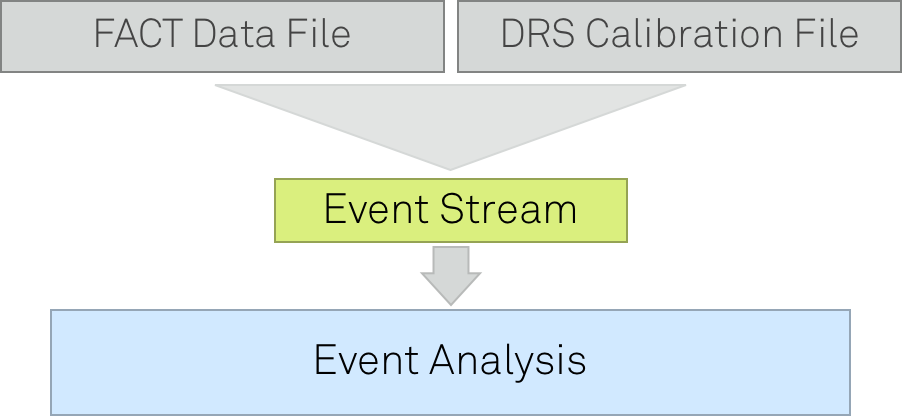
\includegraphics[scale=0.25]{fact-event-stream}
\end{center}
\caption{\label{fig:eventStream}Stream-lined processing of events.}
\end{figure}

As can be seen in this figure, the basic view of the FACT data is that
of a continuous stream of events. The plugin provides a FACT-stream
operator that allows to open a (compressed) FACT file in FITS format
and also implements the DRS calibration used to calibrate the RAW
data. The outcome is a stream of calibrated event objects.

A {\em DataStreamProcessing} operator can then be attached to that
stream to iteratively process the stream event-by-event. That way,
only a single event is read into main memory at a time.


\subsection*{Single FACT Events}
Each single event that is read from the event stream, contains the
full raw, calibrated measurements of the telescope. Within the FITS
data file, there exists a set of attributes that are associated with
each event. These attributes are fully accessible within the {\em
  DataStreamProcessing} operator by their name. Table \ref{tab:factEventKeys}
lists all the attributes of an event that are currently provided by
the {\em FACTEventStream} operator.
\begin{table}[h!]
\renewcommand{\arraystretch}{1.25}
  \begin{center}
    \begin{tabular}{l|l} \hline
      {\bf Name (key)} & {\bf Description} \\ \hline \hline
      {\ttfamily EventNum} & The event number in the stream \\ \hline
      {\ttfamily TriggerNum} & The trigger number in the stream \\ \hline
      {\ttfamily TriggerType} & The trigger type that caused recording of the event \\ \hline
      {\ttfamily NumBoards} & \\ \hline
      {\ttfamily Errors} & \\ \hline
      {\ttfamily SoftTrig} & \\ \hline
      {\ttfamily UnixTimeUTC} & \\ \hline
      {\ttfamily BoardTime} & \\ \hline
      {\ttfamily StartCellData} & \\ \hline
      {\ttfamily StartCellTimeMarker} & \\ \hline
      {\ttfamily Data} & The raw data array ($1440\cdot 300 = 432000$ float values) \\ \hline
      {\ttfamily TimeMarker} & \\ \hline
      {\ttfamily @id} & A simple identifier providing date, run and event IDs \\ \hline
      {\ttfamily @source} & The file or URL the event has been read from \\ \hline
    \end{tabular}
  \end{center}
  \caption{\label{tab:factEventKeys} The elements available for each event.}
\end{table}

The {\ttfamily @id} and {\ttfamily @source} attributes are added by
the FACT-Plugin itself, all the other attributes are provided within
the FITS data files. The {\ttfamily @id} attribute's value is created
from the {\ttfamily EventNum} and date, e.g. {\ttfamily
  2011/11/27/42/8}, denoting the event 8 in run 42 on the 27th of
November 2011.



\subsection*{Installing the FACT-Plugin}
The FACT-Plugin is an extension for RapidMiner. The RapidMiner
open-source software is written in Java and is available for multiple
environments (Windows, Unix). It can be downloaded from
\url{http://rapid-i.com}.

The FACT-Plugin is a simple Java archive ({\em jar}-file) that can be
found at
\begin{displaymath}
 \mbox{\url{http://sfb876.tu-dortmund.de/FACT/}}
\end{displaymath}
To install the plugin simply copy the latest {\ttfamily FACT-Plugin.jar}
to your RapidMiner {\ttfamily lib/plugins} directory. After restarting
RapidMiner, the plugin will be loaded and all of its additional operators
will show up in the operators list.




\subsection{Concept}



\section{\label{sec:operators}FACT-Plugin -- Operators}


\section{\label{sec:examples}Example Processes}

\begin{figure}[h!]
  \begin{center}
    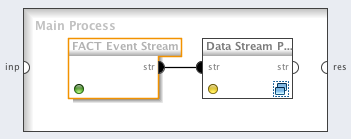
\includegraphics[scale=0.6]{event-stream-process}
  \end{center}
\caption{\label{fig:event-stream-process}Top-level view of a RapidMiner experiment including an FACT event stream}
\end{figure}

%\begin{abstract}
%% Short abstract of your report
%\end{abstract}



% Bibliography using Bibtex, style plain
\bibliography{TechReport}{}
\bibliographystyle{plain}

\end{document}
